




% Antar begreper qknn har blitt intodusert

Now that a parallel k-d tree build algorithm has been build, lets start looking into a parallelization of the qkNN operation. Some question immediately arise. What is the best way to parallelize such a problem? Will a GPU version give a beneficial speedup? This leads to a new research question that acts as an extention of RQ~\ref{rq:serial-kd-tree}.


\begin{myrq}
\label{rq:parallel_query}
    It is possible to parallelize the qkNN query algorithm, in such a way that it gives a significant speed improvement compared to the serial algorithm.
\end{myrq}


To investigate RQ~\ref{rq:parallel_query}, a real world test and implementation is always beneficial, but first some resource and discussion is needed. Especially in what kind of parallelization strategy and algorithm that should be used. Maybe the GPU is not the right way to parallelize this kind of operations.


\subsection{Parallelization strategy} % (fold)
\label{sub:parallelization_strategy}


The problem at hand is the qkNN search, which is where an assumed big number of query's is to be performed on a k-d tree. At first glance this looks good in terms of parallelization. The main task is naturally divided into individual subtasks, namely the queries. This is a perfect parallelization example, where any number of threads independently can move up and down a constant tree structure.

However, there are steal some interesting aspects that should to be addressed. The first is how the work should be divided in terms of CUDA resources. Should a query be done in one block, maybe each query should be done single handedly by one thread, or maybe we should use one thread per $k$ in a query. To address this question, one need to be able to determined if a query itself can be parallelized and what kind of resources that is available.

First we see that a query does not have many node visits compared to the size and presumably the number of queries in a search. This ratio is based on the binary logarithm. For example would a qkNN operation on a tree with one million elements and a $k$ equals one, visit proportionally $20$ nodes. This indicated that many threads per query is not very beneficial, because they should be used to query other points. 

The relative hard problem of parallelize a query is also a good indicator. Parallelization is, as we have discussed earlier, dependent on individual and dividable subtasks. The query task is heavily dependent, because the next node in the search traversal is determinant on the previous node. The only thing that could be parallelized is if we wanted to search both left and right subtree simultaneously, but if this is parallelized the benefit of the pruning is partially destroyed. This leads to one conclusion, if threads is not to be wastefully used, one thread per query is the natural choice. In terms of independent tasks, the one thread approach is also logical, since the number of queries should outperform the number of cores on the GPU\@.

The overall parallelization strategy is therefore to use one thread per query and equally distribute the queries amongst the GPU's SM\@.


\subsection{Problem with the recursive implementation} % (fold)
\label{sub:problem_with_the_recursive_implementation}

As discussed in previous sections, GPU's and recursion don't get along well. Previously some drawbacks were mentioned, including the disability for thread communication. Since our parallelization strategy now states that all threads do individually work and don't need to communicate, are there steal reasons for why the recursive implementation not should be used.

One aspect to consider is connected to how the GPU hardware is constructed. The GPU have a lot of lightweight threads, and has therefor not as mush local space or caching as in a CPU\@. This means that the call stack, where the instructions are managed, is relatively small. A recursive algorithm adds instructions on this call stack at each recursive call. This is the reason why the executions flow of a recursive algorithm is hidden, or in other words not reachable from the programmers point of view. The big question is wherever the call stack on a CUDA GPU is big enough for our application.

This question was investigated by a trail and error method, since its hard to do the explicit calculations. The call stack is located locally on each thread, so investigations on one block should be enough. To test the limitations a test that spawned $64$ theoretical threads on an increasing tree size should be sufficient. The results showed that when the tree size passed \numprint{1e5} points, unknown errors started to appear. This was probably the leak of call stack space and it was concluded that CUDA had a to small call stack for our purpose.

Divergence is also an accept to consider, and in this case execution divergence. This is, as mention before, then the execution of threads in a warp differs. In a recursive algorithm the decision of whether a recursive call should be made or not, is entirely up to a single thread and the execution stack may then be asynchronous. Once two threads have made different decisions, there is no guaranty that they will stay in sync.

The execution divergence can be solved by en iterative solution, where one is guaranteed that every thread always stay in sync. An iterative approach will also solve the call stack problem, where the recursion stack is explicitly stored. The transformation from a recursive to a iterative algorithm is therefore a necessity.


% subsection problem_with_the_recursive_implementation (end)

\subsection{From recursive to iterative implementation} % (fold)
\label{sub:from_recursive_to_iterative_implementation}


To rewrite Algorithm~\ref{alg:recursive_knn_kd_tree_search} into a iterative algorithm by explicitly managing the recursion stack, some properties about how the search traverse the k-d tree is needed. From Algorithm~\ref{alg:recursive_knn_kd_tree_search} one can see that this is an inorder traversal, since the work of the current node is done between the recursive calls. This traversal in also the best strategy in a binary tree search, because the pruning of subtrees is maximized. How to make a standard binary search tree in an iterative fashion is described in Cormen\citep[Chapter 12]{Cormen:2001}, but since this is a k-d tree search the implementation is slightly different, as shown in Algorithm~\ref{alg:iterative_knn_kd_tree_search},

\begin{algorithm}
\caption{Iterative kNN k-d tree search}
\label{alg:iterative_knn_kd_tree_search}
\begin{algorithmic}
    \Procedure{Iterative-kNN-KD-Tree}{$K, r, q$}
        \State \text{Let $S$ be a stack for collecting tree nodes}

        \State $i \gets 2$

        \While{$!S.empty$ \textbf{or} $r$ != NIL}
            \If{$r$ = NIL}
                \State $r \gets \Call{Pop}{S}$
                \State $i \gets r.dimension$

                \If{$r.dx^2 < K.max$} \Comment{Can there be closer points in the other subtree?}
                    \State $r \gets r.other$
                \Else
                    \State $r \gets \text{NIL}$
                \EndIf
            \Else
                \State $d \gets \Call{Distance}{r, q}$

                \If{$d < K.max$} \Comment{Is $r$ closer to $q$ than the current k best points?}
                    \State $r.distance \gets d$
                    \State $\Call{Insert}{K, r}$
                \EndIf

                \State $i \gets (i + 1) \bmod k$ \Comment{k = 3 for a three dimensional k-d tree}

                \State $r.dimention \gets i$
                \State $r.dx \gets r.x(i) - q.x(i)$

                \If{$r.dx > 0$}  \Comment{Select $t$ and $o$ so we traverse towards closest point first}
                    \State $t \gets r.left$, $r.other \gets r.right$
                \Else
                    \State $t \gets r.right$, $r.other \gets r.left$
                \EndIf

                \State $\Call{Push}{S, r}$
                \State $r \gets t$
            \EndIf

        \EndWhile
    \EndProcedure
\end{algorithmic}
\end{algorithm}

The algorithm works in the same way as the recursive algorithm, but adds a stack, $S$, called the s-stack, and a while loop in order to handle the tree traversal iteratively. While there is a element assigned to the root variable, $r$, the algorithm will traverse down the target branch, updating the dimension, $i$, calculating the distance, $dx$, determining the target, $t$, and other, $o$, child node. Then it will collect $r$, $o$, $i$ and $dx$ into one element, and push it on the s-stack. Finally the root variable is assigned to the target child, or NIL if we have reached the end of a branch.

While there still is elements in the s-stack, but $r$ is assigned to NIL, we are traversing back up a branch. While this is happening, the algorithm pops elements from the s-stack, determines if they should be added to the k-heap, before it determines if it need to investigate the other branch of this node. If that is the case, the other node is assigned to $r$, and the algorithm will traverse down this subtree using the previously stated rules.


% subsection from_recursive_to_iterative_implementation (end)

%TODO: Forandre header?
\subsection{CUDA implementation} % (fold)
\label{sub:the_implementation}

To convert our iterative search algorithm to CUDA should, because of Algorithm~\ref{alg:iterative_knn_kd_tree_search}, be a trivial matter. The code itself does not need to be parallelized, as only one thread is used per query. The final implementation can be found in Appendix~\ref{sec:cuda_k_d_tree_search}. However, some key aspects is wort highlighting.


As we converted the algorithm from a recursive to a iterative stack based solution, a lot of the problematic divergence was taken avoided. But as shown in Algorithm~\ref{alg:iterative_knn_kd_tree_search}, there is steal some divergence. This is inevitable, since the target subtree and other subtree needs to be treated differently. Although, there are possibilities to minimize the thread branching. If threads in a warp is traversing completely different parts of the tree, they will access different nodes. This is called data divergence. The solution is to let each warp search for points that are close in 3-d space, which will force the threads to traverse more or less together down the tree. In our application, querying for all points in the k-d tree, this is an easy task. When the k-d tree was build the points where, due to the data structure and the nature of a k-d tree, grouped together relatively to their position in space. The divergence will therefore be minimized if the points are fed to the search algorithm as they are placed in the k-d tree.


The explicit stack also makes an interesting question about where to store the new stack. This is data that are modifiable and thread independent, which means that the most trivial memory options are shared memory, local memory and global memory. Local memory is the memory each thread can allocate dynamically from the heap. First of all, global memory is a working candidate. It has enough space, it is modifiable and accessible to all threads. The huge drawback is the access time, it takes around $400-600$ clock cycles(Trenger vi cite), and it would therefore be beneficial to use some other kind of memory. Shared memory would be a perfect candidate, because the memory is fast and the need to communicate between blocks is nonexistent. The only drawback is the amount of data available in shared memory, which is around $49 kb$ on current NVIDIA GPU's. 


(Results from k-stack varitation, and rewrite sectionsta under)

The two stacks in question is the k-stack and the transformed recursive stack, called s-stack from now on. Both stacks are memory wise dependent on the number of threads in use, since each thread needs unique stacks. The s-stack is dependent on how many elements the inorder tree traversal needs to store. If one looks on how the algorithm handles the stack, one can see that elements are pushed on the way down, and poped on the way up.  This means that the stack never will be longer then the tree hight. One stack element uses $16$ bytes of space, which means that the stack memory is s subset of $\Theta(16\log_2(n)T)$. Here $T$ represent the number of threads and $n$ is the k-d tree size. The k-stack depends on the number of closest neighbors, $k$, and one element uses $8$ bytes. This implies that it's memory usage will look like, $\Theta(8kT)$.


\begin{figure}[ht!]
\centering
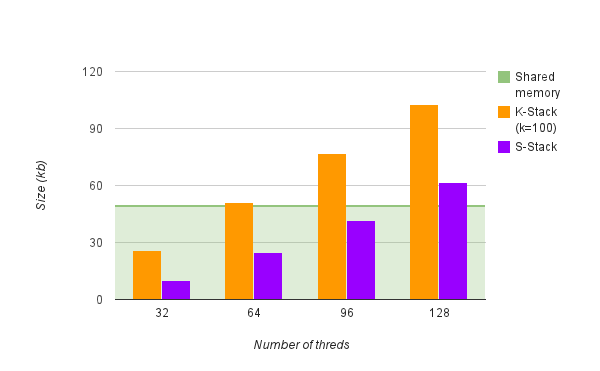
\includegraphics[width=100mm]{../gfx/shared_memory_and_stack.png}

\caption{The stacks memory usage, compared to the amount of shared memory. Here $k$ was sat to $100$.}
\label{fig:stacks_and_shared_memory}
\end{figure}


In Figure~\ref{fig:stacks_and_shared_memory} the memory usage of each stack is compared to the available shared memory. Some basic assumptions and approximations have been done in regard to the data. Treads are only compared in multiples of $32$, since this is the warp size and is therefore the most optimal thread numbers. The value of $k$ is dependent on the problem in hand, and as our application only needs a value of $100$, so that value is used. 


Figure~\ref{fig:stacks_and_shared_memory} shows that the k-stack is not a suitable candidate. Already at a thread count of $64$ the memory is filled up. The highly dependent and variably $k$ value also make the stack size unpredictable. The s-stack however looks really promising, with $64$ threads the memory usage is well below the limit. The memory size has also a relatively low asymptotic growth, \BigO{log(n)}, in regard to the tree size.

\begin{figure}[ht!]
    \centering
    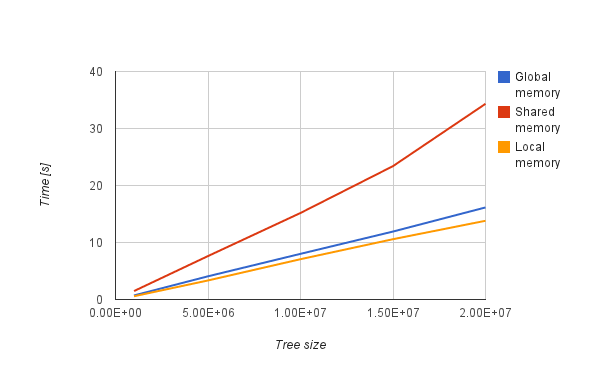
\includegraphics[width=100mm]{../gfx/stack_speed.png}

    \caption{Speed comparison between different stack memory types. The test are done with $k$ equals 10 and \numprint{1e6} queries per tree size. }
    \label{tbl:stack_speed}
\end{figure}



To decide what kind of memory is optimal for our stack, Figure~\ref{tbl:stack_speed} has been created. Surprisingly shared memory looks like the slowest alternative. One likely reason is that elements in shared memory is synced between all threads in a block. This property is not needed in the s-stack, since the s-stack is only used by one thread. 


% Skal vi ha med denne?
An other reason is that there is some kind of programming error, and some part of the s-stack is used by two threads. This would lead to a lot of write and read collisions, and cause a lot of time penalties. The programming error would also lead to wrongly results, which is not the case and the error possibility is ignored.

Although global and local memory presumably is stored at the same place, the are some noticeable differences that can explain the time gap between them. The cache may be a factor. The cache is placed on the same on-chip memory as the shared memory, and should therefore be equally fast. The difference is that cashing is not programmable and therefor not controlled be the programmer. However some properties in the local memory may suggest that it is a more likely candidate to be cached. The local memory is thread dependent and is not accessible to other threads or blocks as the global memory are. The compiler can therefor logically imply that the data is not going to be modified by other threads and caching becomes mush more likely. Figure~\ref{fig:stacks_and_shared_memory}, also shows us that the cache can fit the hole s-stack in a block, which correlates with the timing results. To enforce cache use even further, CUDA gives a runtime option to enforce more of the on-chip memory to caching.


\begin{figure}[ht!]
    \centering
    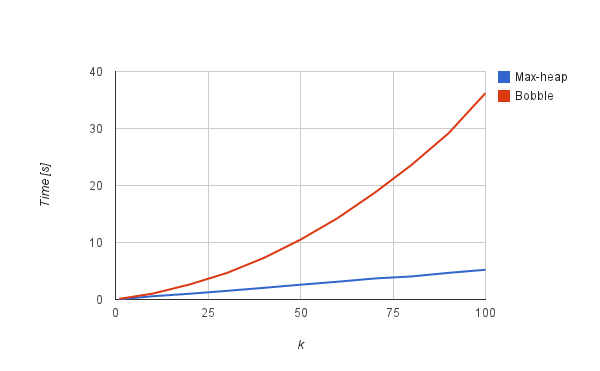
\includegraphics[width=100mm]{../gfx/k_stack.png}

    \caption{Timing results from two different k-stack implementations, with varying $k$ and \numprint{1e6} referance points. }
    \label{tbl:k_stack}
\end{figure}


% Må ha Skal vi ha noen diskusjon rundt k-stack. 
The discussion and results for the stack analysis shows that the stacks highly impact the timing results. This means that the k-stack is also a dominant  speed factor, as corresponds well to the k-stack tests, shown in Figure~\ref{tbl:k_stack}. Two k-stack variants was tested. One that used a bobble sort\cite{Cormen:2001} like implementation. It works by always keeping a sorted list. Elements are inserted by placing it at the end if the list, and swapping it to the adjustment element, until it is in the right place. The other method is based on a heap sort implementation, that is explained in Section~\ref{sub:querying_the_k_d_tree}. The difference is the insertion time, where the bobble variant is a \BigO{n} time complexity, while heap sort variant has a \BigO{log_2(n)}. Resulting in a almost $7$ times baster k-stack, with only a $k$ value of $100$, mostly because the max-heap variant needs lesser element retrievals. (TODO: Skrive om dette lite jaaaaa)


\subsubsection{Open-MP} % (fold)
\label{ssub:open_mp_version}

The high impact the stack had on performance make an interesting question in regard to RQ~\ref{rq:parallel_query}. Could a parallel implementation in the CPU outperform the CPU version? When the latency effect, as the stacks showed, had such a huge impact on the performance. The CPU has a lot more cache then the GPU and would therefor not be affected that mush. The real question is whether the CUDA implementation manges to hide the latency problem by alternating between different warps.

For this to be investigated properly, an OpenMP version of the k-d tree search has to be created. Parallelization wise this is not as different as in our CUDA discussion, and there are only some implementation details to address. The big discussions around what kind of memory to use or memory size can also be ignored, since the CPU has enough cache and the latency is not that important. The implementation can be found in Appendix~\ref{sec:open_mp_k_d_tree_search}.

% subsubsection open_mp_version (end)


% subsection our_implementation (end)











% \begin{figure}[ht!]
% \centering
% 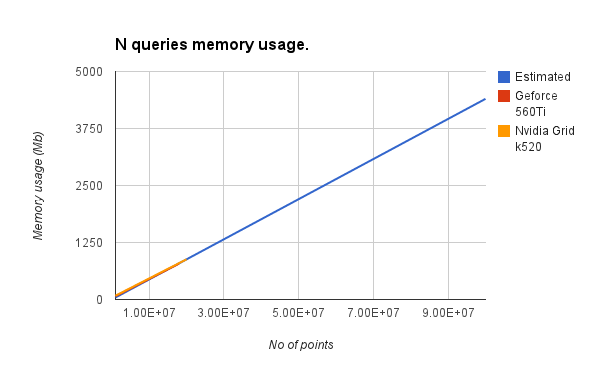
\includegraphics[width=120mm]{../gfx/memory-usage-kd-search.png}

% \caption{Memory usage of kd-search.}
% \label{fig:memory-usage-kd-search}
% \end{figure}

% Also in this case our estimation fit the real consumption with a high degree of accur
% Further work:
% \begin{itemize}
%     \item Look at memory optimization.
%     \item Improve utiliti methods like: accumulateindex, minReduce.
%     \item Forloop Unrolling.
% \end{itemize}



